%# -*- coding: utf-8-unix -*-
%%==================================================
%% chapter01.tex for SJTU Master Thesis
%%==================================================

%\bibliographystyle{sjtu2}%[此处用于每章都生产参考文献]
\chapter{系统实现}
\label{chap:sys_implement}

上一章介绍了系统的设计,这一章将首先介绍系统实现所需的预备知识,进而介绍系统的具体实现。

\section{预备知识}

由于系统位于linux内核态,因此需要对内核中与系统实现相关的基本知识进行介绍。这些预备知识包括Linux存储层次、bio、Device Mapper等。

\subsection{Linux存储层次}

Linux存储层次如图\ref{fig:linux_storage_layer}所示,大致可分为共六层\cite{敖青云2011存储技术原理分析}:

\begin{enumerate}
    \item 最上层位于用户态,对用户看到的文件,用户的应用程序通过调用POSIX接口对这些文件进行操作。

    \item 第二层为虚拟文件系统(VFS, virtual file system)层,位于内核态。VFS的作用为屏蔽其所管理的具体文件系统,使用户可以使用统一的接口进行调用。POSIX在VFS层将数据封装成bio,然后将bio交给挂载的具体文件系统执行操作,bio将在\ref{sec:bio}具体介绍。

    \item 第三层为块层(block layer),位于内核态。块层负责将bio封装成设备请求(request)。具体封装方法为:如果几个bio的读写区域连续,那么将他们积攒成一个request,request下挂多个连续bio,即合并bio请求。如果bio跟其它bio都不连续,则它自己创建一个新request,将自己挂到这个request下。每个request下能挂的bio有限,多个连续bio的访问总区域超过一定限额,就不能合并为一个request。之所以不将多个bio合并为一个bio而是使用request,是因为每个bio都有自己的回调,如果合并为一个bio则失去了对不同bio使用不同回调的灵活性。合并后的request会以队列的形式组织起来,等待SCSI层进行处理。

    \item 第四层为SCSI层,位于内核态。SCSI层负责将request封装成与块设备具体存储格式相关的SCSI命令。

    \item 第五层为设备驱动(device driver)层,位于内核态,负责接收SCSI命令,并将其转换为设备请求,将其放入设备请求队列。

    \item 第六层为具体的设备层,位于内核态,负责接收设备请求,并在实际设备上执行对应的操作。

\end{enumerate}

\begin{figure}[!htp]
    \centering
    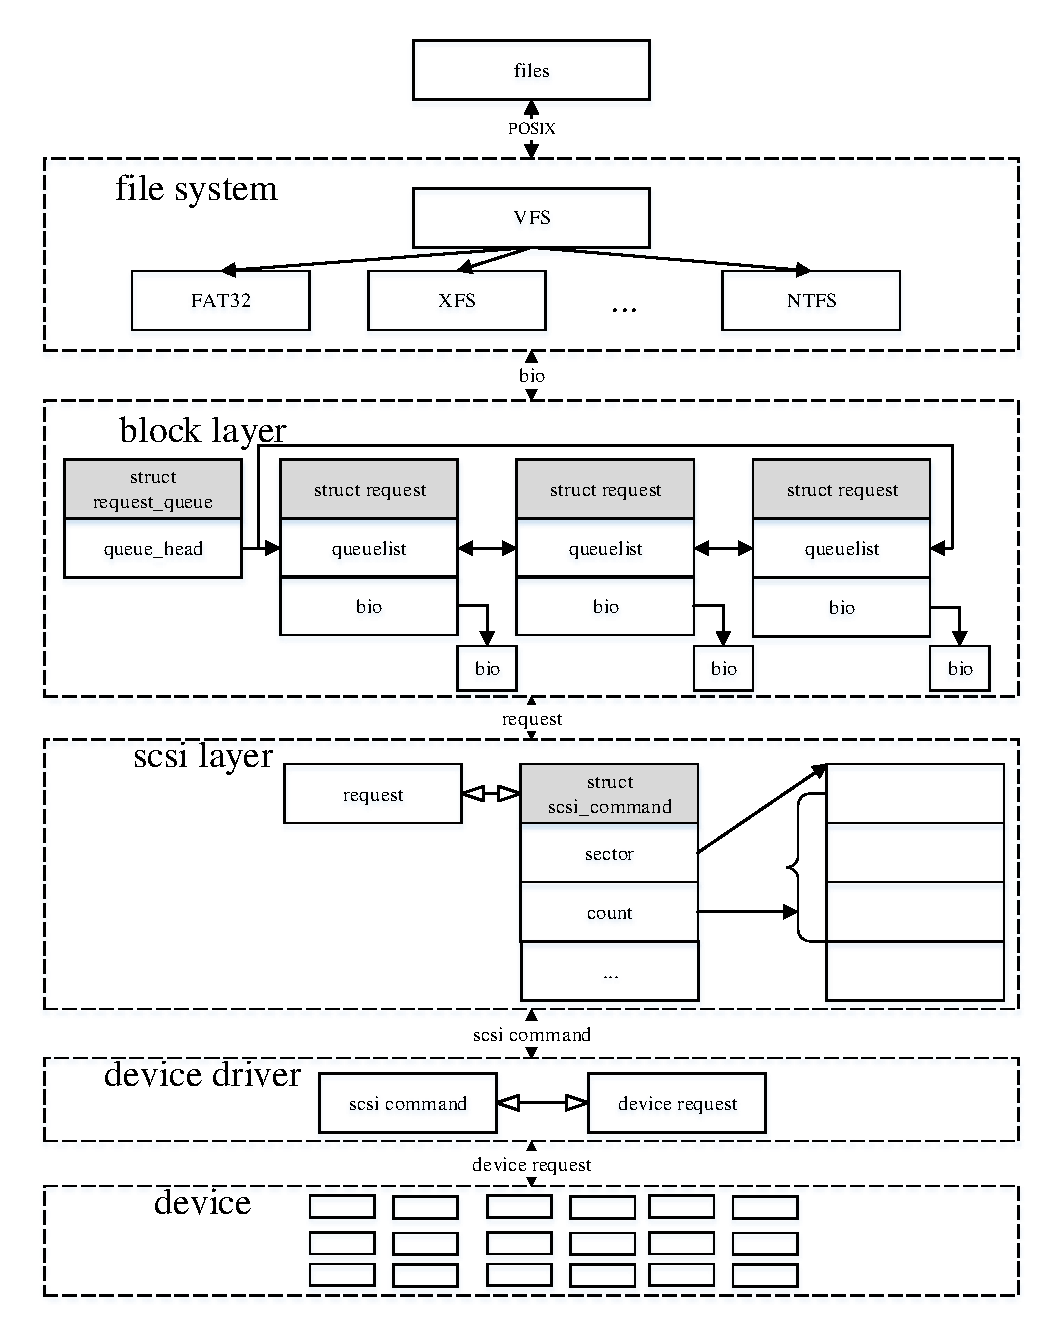
\includegraphics[width=\textwidth]{linux_storage_layer.pdf}
    \bicaption[fig:linux_storage_layer]{Linux存储层次}{Linux存储层次}{Fig}{linux storage layer}
\end{figure}

\subsection{bio}
\label{sec:bio}

bio这一数据结构被用来描述块设备的I/O操作,将内存缓冲区与块设备联系起来的重要桥梁\cite{corbet2005linux}。

bio的具体结构如图\ref{fig:bio}所示。一个bio指针指向由bio结构体组成的链表,bio结构体中的bi\_io\_vec指向一个bi\_vec结构体数组,每个bi\_vec结构体中bv\_page指向内存中的实际页,bv\_offset和bv\_len组合来定位数据在该页中的具体位置,如此,一个bio链表就将散落在内存中的各数据组织为一个块设备请求。

\begin{figure}[!htp]
    \centering
    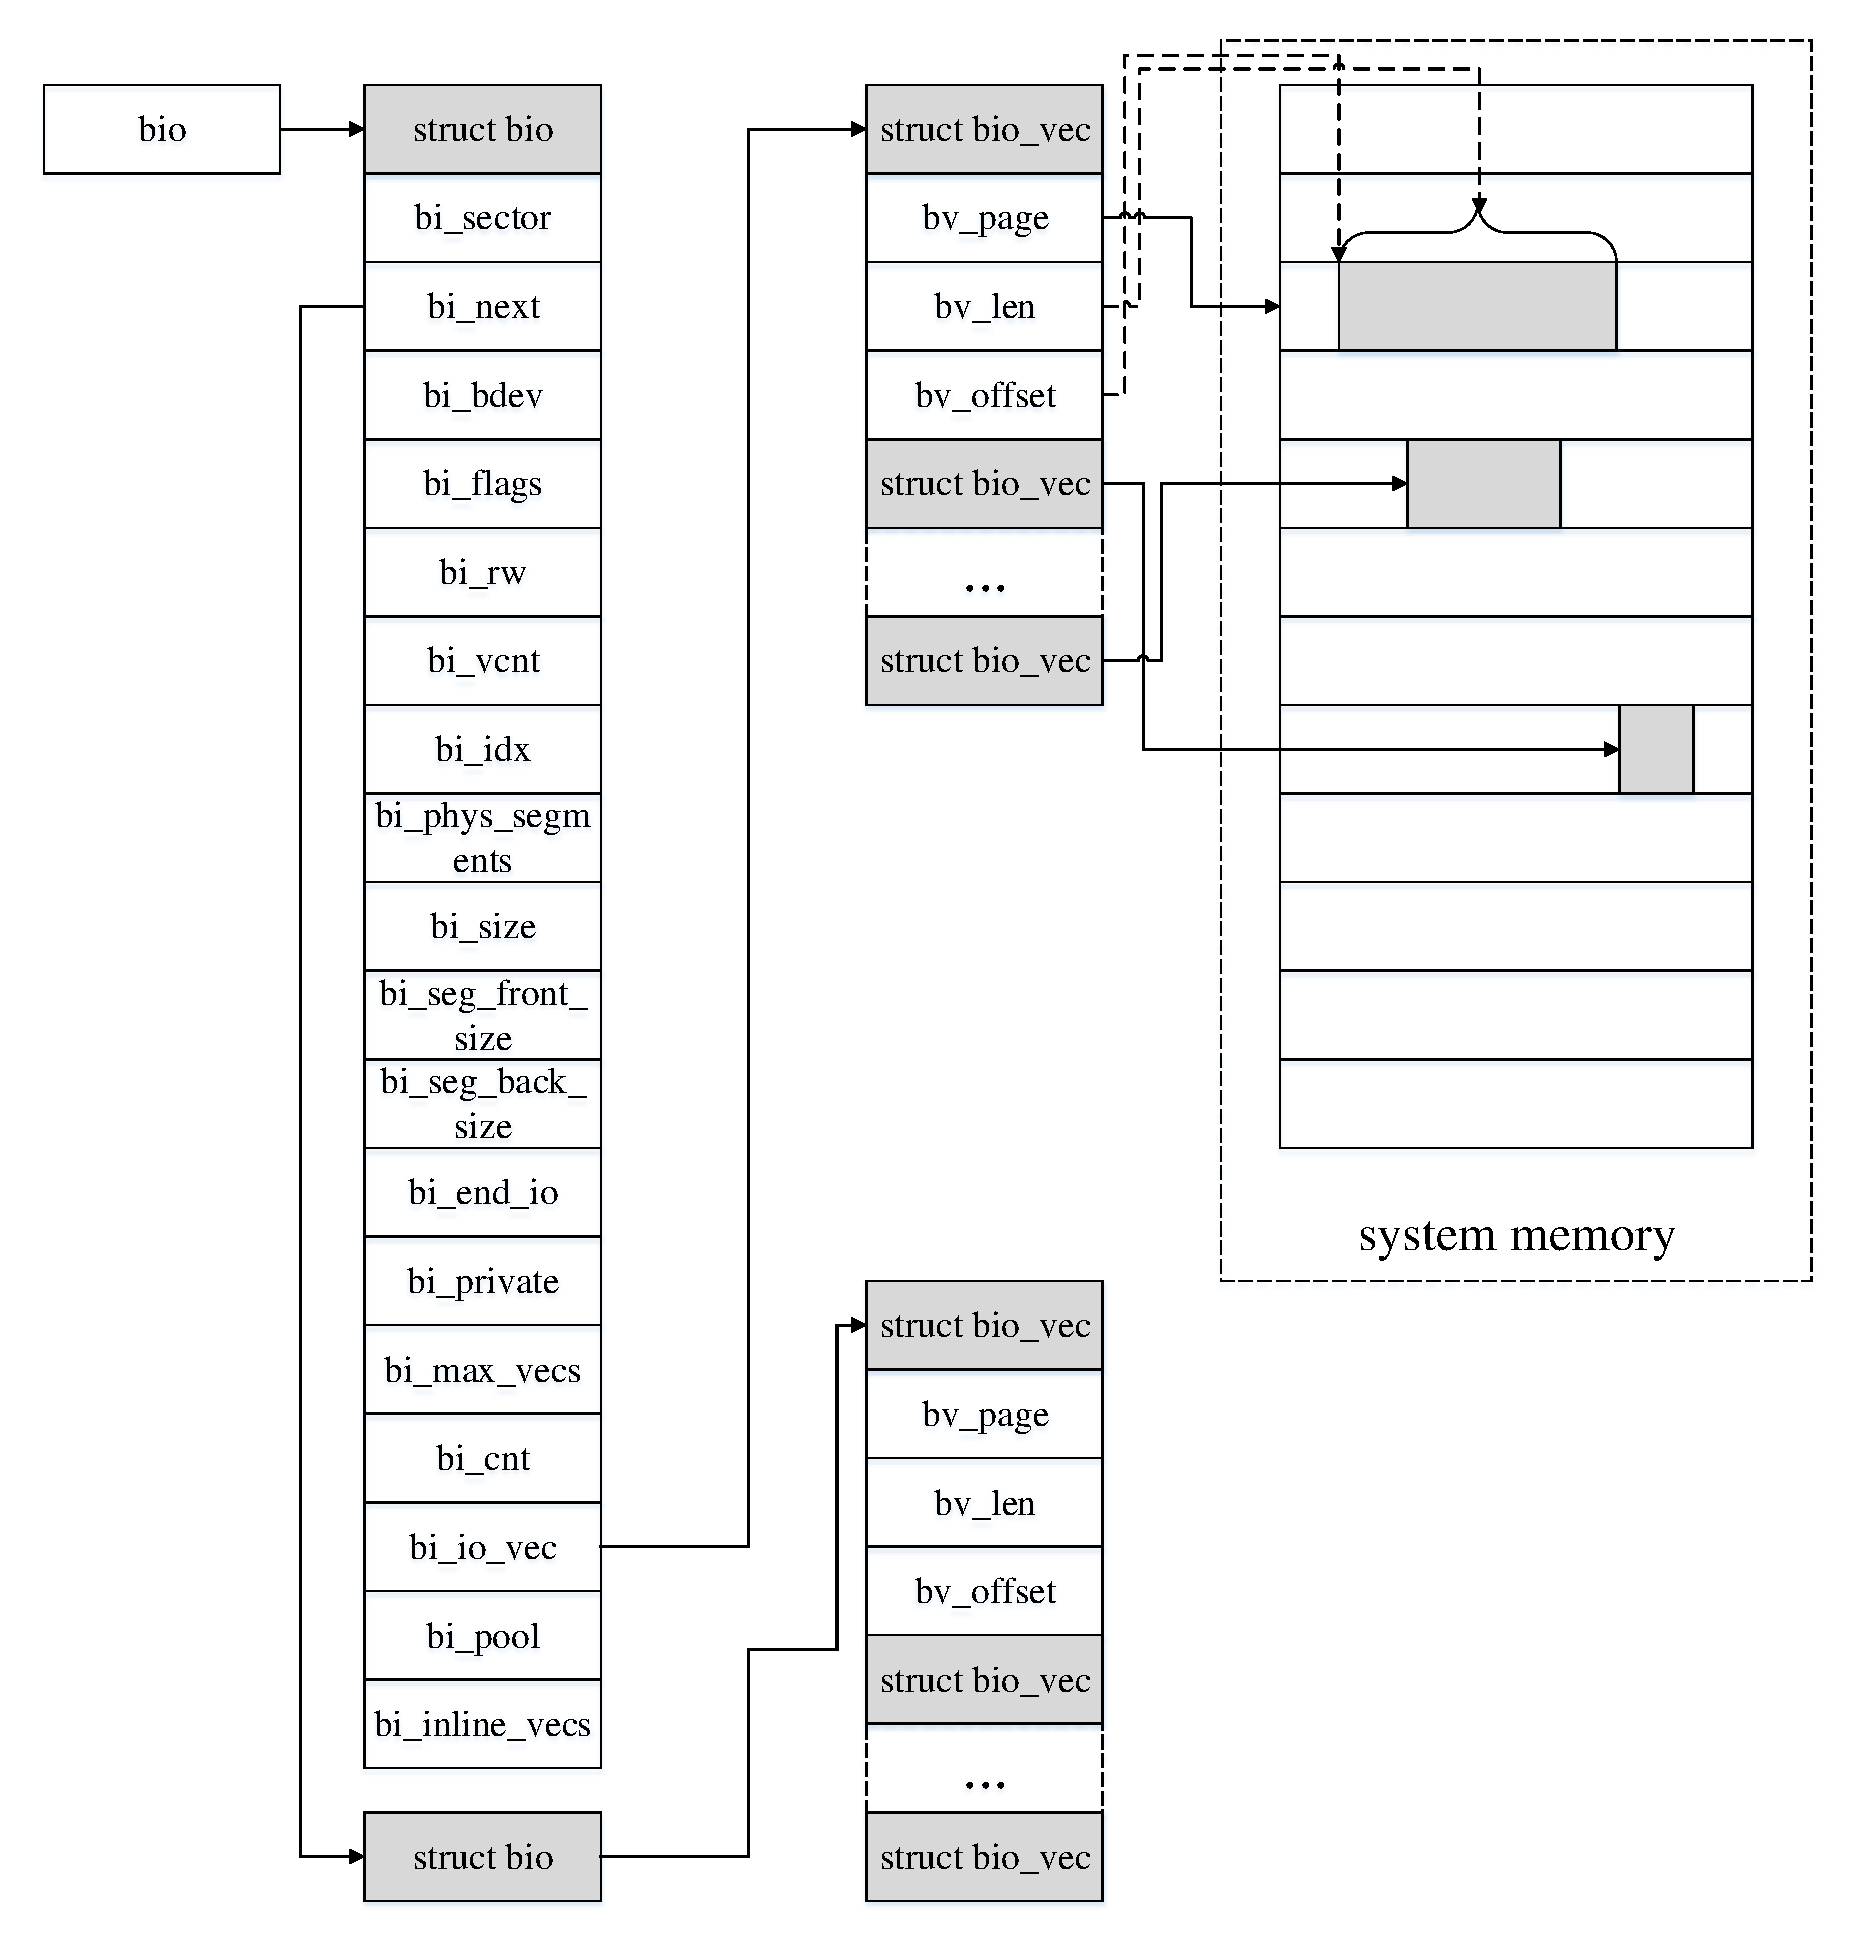
\includegraphics[width=0.8\textwidth]{bio.pdf}
    \bicaption[fig:bio]{bio结构}{bio结构}{Fig}{bio structure}
\end{figure}

\subsection{Device Mapper}

Device Mapper是Linux2.6 内核中支持逻辑卷管理的通用设备映射机制,它为实现用于存储资源管理的块设备驱动提供了一个高度模块化的内核架构\cite{bovet2005understanding}。Device Mapper以一个块设备驱动在内核中注册,它包含mapped device、mapping table、target device这三个重要概念。mapped device可以理解为内核对外提供的逻辑设备,用户看到的也是这个逻辑设备,mapped device通过mapping table组织与与target device的映射关系,一个mapped device可以映射到一个或者多个target device上,总体层次如图\ref{fig:device_mapper}所示,target device可以是真实的物理设备也可以是另一个mapped device,如此迭代,形成一个树状结构。

\begin{figure}[!htp]
    \centering
    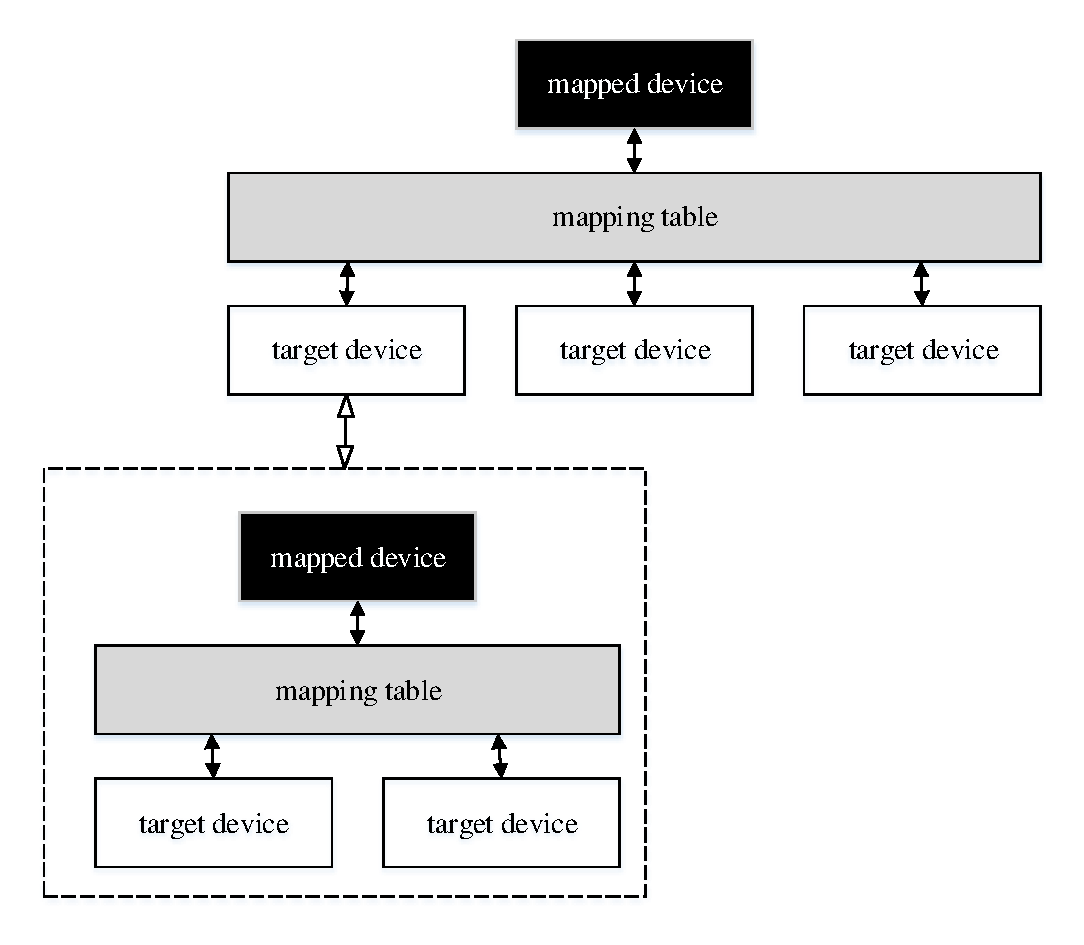
\includegraphics[width=0.8\textwidth]{device_mapper.pdf}
    \bicaption[fig:device_mapper]{Device Mapper层次图}{Device Mapper层次图}{Fig}{Device Mapper Layer}
\end{figure}

Device Mapper的实现原理是将mapped device的make\_request\_fn方法实现为自己的dm\_request,这个经过mapped device的bio请求都会进入dm\_request方法,之后Device Mapper通过判断mapped device是基于request还是基于bio来分别处理:

如果mapped device是基于request的,那么和磁盘设备一样通过generic\_make\_request把bio合并为request,将其放到mapped device的request队列中,当mapped device通过kblockd调用dm\_request\_fn时,dm\_request\_fn中会调用peek\_request从mapped device的request队列中拿出request将其clone(clone生成的request中的bio与原request中的bio指向同一个内存页,clone操作只是分配新的bio和request),然后通过调用map\_request将request映射,将clone后的request发往低层的真实设备。

如果mapped device是基于bio的,那么调用\_dm\_request首先clone bio然后调用\_\_map\_bio将bio映射,将clone后的bio通过generic\_make\_request发往低层的真实设备。

mapped device基于request还是基于bio的主要区别在于,如果是基于request则request是放在mapped device的request队列中,如果是基于bio,则是在调用generic\_make\_request总将bio封装成request放到真实设备的request队列中。


\subsection{其他预备知识}

在系统的实现过程中,除了上面介绍的几个关键知识点外,还涉及很多其他的Linux内核知识,比如Linux的内核模块编程、内核编程中的常用宏、常用数据结构、内核的调试等内容,这里不再详细介绍。

\section{编程实现}
\section{本章小结}